\section{Local Visual Object Position Is Not Sufficient}
\label{sec:sufficiency}

The reach-field result is correlational: under displacement, the reach points at $\Cv$. But \emph{why}? One hypothesis is that the agentview object position drives the endpoint, and displacement simply moves it out of a learned in-distribution band. If so, then \emph{showing} the object at a location should move the reach there. We test this with a causal intervention.

\paragraph{Renderer-local object paste.} A naive test---translating the entire observation frame---is itself out-of-distribution for the policy (in pilot runs a global frame translation broke $87\%$ of otherwise-healthy episodes), so it cannot cleanly adjudicate sufficiency. Instead we move only the object's \emph{appearance}: at each policy step we save the target object's pose, kinematically set it to a \emph{visual} location $V$, re-render the cameras, restore the true pose, and feed the policy the re-rendered image while stepping the real physics. This changes only the object's $\sim$2k rendered pixels (both agentview and wrist), leaving the rest of the scene---and the real physics---intact (a no-op sham render changes $0$ pixels, confirming the machinery is identity when $V$ equals the physical location).

\paragraph{Design.} We cross physical and visual object location in a $2{\times}2$ factorial plus a specificity control, at $50$\,mm on the clean-success pairs: \textbf{CC} (physical $\Cv$, visual $\Cv$; sham), \textbf{CT} (physical $\Cv$, visual $\Tv$; the primary sufficiency arm), \textbf{TC} (physical $\Tv$, visual $\Cv$), and \textbf{CR} (physical $\Cv$, visual $\Cv+R_{90}\dv$; a specificity control that pastes the object at an orthogonal $90^\circ$ visual displacement). The sufficiency statistic is the endpoint shift from sham toward the pasted location, $S=\langle\Ev_{CT}-\Ev_{CC},\dv\rangle/\lVert\dv\rVert^2$; $S\!\approx\!1$ means the reach follows the visually-pasted object, $S\!\approx\!0$ means it ignores it.

\paragraph{Visual position does not steer the reach.} Over the full $740$-rollout grid, showing the object at a false location does not move the reach (\cref{fig:e2r}). The endpoint shift toward the pasted location is null: $S_{CT}$ has median $+0.06$ (task-cluster bootstrap $[-0.02,+0.12]$), only $32\%$ of CT endpoints are closer to the visually-pasted $\Tv$ than to $\Cv$, and the orthogonal specificity control is likewise inert ($S_{CR}=-0.04$). The success pattern is decisive and precision-independent: grasp success tracks the \emph{physical} object position and is indifferent to the \emph{visual} one. With the object physically at $\Cv$, showing it displaced barely changes success (\textbf{CT} $72\%$, $106/148$, vs.\ sham \textbf{CC} $75\%$, $111/148$); with the object physically at $\Tv$, showing it back at $\Cv$ does not help (\textbf{TC} $30\%$, $44/148$, vs.\ \textbf{TT} $32\%$, $48/148$). In \textbf{CT} the policy grasps the object at its true canonical location despite seeing it elsewhere---if the rendered position steered the reach, CT would aim at $\Tv$ and fail. The reach endpoint is thus decoupled from the agentview object position, both its real and its visually-pasted value.

\begin{figure}[t]
\centering
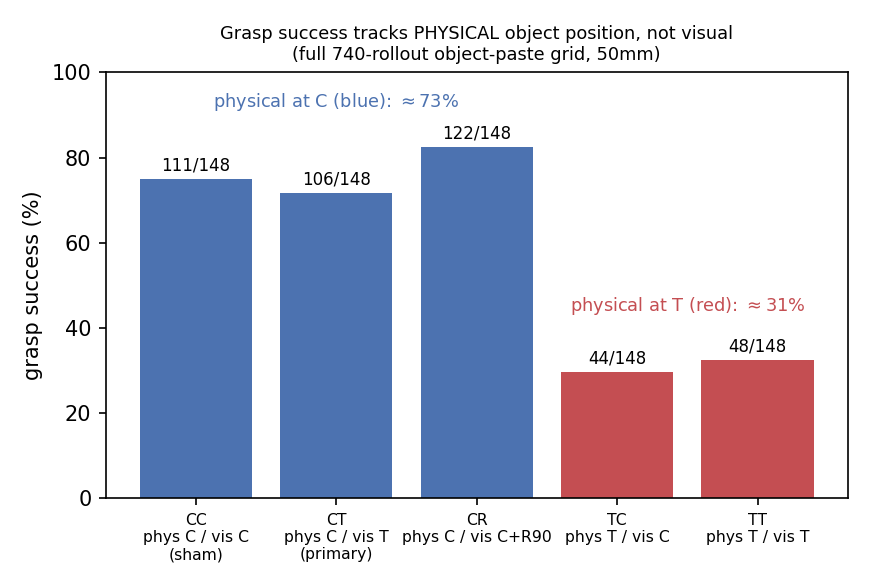
\includegraphics[width=0.55\textwidth]{figures/fig_e2r.png}
\caption{\textbf{Object-local paste intervention (full $740$-rollout grid, $50$\,mm).} Grasp success by condition (counts above bars), colored by \emph{physical} object location. Success tracks the physical position (at $\Cv$: CC/CT/CR $\approx 73$--$82\%$; at $\Tv$: TC/TT $\approx 30\%$) and is indifferent to the \emph{visual} position: CT (physical $\Cv$, shown $\Tv$) $\approx$ sham CC, and TC (physical $\Tv$, shown $\Cv$) $\approx$ TT. Showing the object elsewhere does not move the hand there.}
\label{fig:e2r}
\end{figure}

\paragraph{Interpretation.} Taken with \cref{sec:competent}, two manipulations that place the object's appearance away from $\Cv$---a real displacement (E1r) and a visual paste to a false location (CT)---both leave the reach endpoint aimed at $\Cv$, while pasting a displaced object's appearance back at $\Cv$ (TC) fails to rescue the displaced physical task. The endpoint is consistent with a canonical prior decoupled from the current agentview object position, rather than tracking it. We reserve the ``not sufficient'' claim to exactly this intervention: local rendered object position does not steer the reach in this setting. The CT-vs-TC success contrast is decisive independent of endpoint precision.
